\documentclass[journal]{IEEEtran}
\usepackage{cite}
\usepackage{amsmath,amssymb,amsfonts}
\usepackage{graphicx}
\usepackage{textcomp}
\usepackage{xcolor}
\usepackage{colortbl}
\usepackage{url}
\usepackage{booktabs}
\usepackage{multirow}
\usepackage{tikz}
\usepackage{pgfplots}
\pgfplotsset{compat=1.17}
\usetikzlibrary{shapes.geometric, arrows.meta, positioning, fit, backgrounds, calc, patterns, shadows.blur}
\providecommand{\bibname}{References}

%% Professional IEEE Color Palette
\definecolor{IEEENavy}{RGB}{0,51,102}
\definecolor{IEEEBlue}{RGB}{0,102,204}
\definecolor{IEEELightBlue}{RGB}{204,229,255}
\definecolor{IEEETeal}{RGB}{0,128,128}
\definecolor{IEEELightTeal}{RGB}{204,242,240}
\definecolor{IEEEGreen}{RGB}{0,120,60}
\definecolor{IEEELightGreen}{RGB}{204,240,220}
\definecolor{IEEEOrange}{RGB}{200,80,0}
\definecolor{IEEELightOrange}{RGB}{255,220,180}
\definecolor{IEEEPurple}{RGB}{90,0,140}
\definecolor{IEEELightPurple}{RGB}{230,200,255}
\definecolor{IEEERed}{RGB}{180,0,0}
\definecolor{IEEELightRed}{RGB}{255,210,210}
\definecolor{TableHeader}{RGB}{0,51,102}
\definecolor{TableAlt}{RGB}{235,242,252}
\definecolor{ASCENDLayer1}{RGB}{0,80,160}
\definecolor{ASCENDLayer2}{RGB}{0,110,90}
\definecolor{ASCENDLayer3}{RGB}{180,70,0}
\definecolor{ASCENDLayer4}{RGB}{100,0,140}


\documentclass[conference]{IEEEtran}
\usepackage{hyperref}          % Enables clickable links
\hypersetup{
    colorlinks=true,
    linkcolor=black,
    filecolor=black,      
    urlcolor=blue,
}

\begin{document}

\title{Multi-Track Deployment, AI-Powered Post-Deployment Synchronization in Enterprise CI/CD}

\author{
  % ── AUTHOR ───────────────────────────────────────────────────────────────
  \IEEEauthorblockN{Venkata Pavan Kumar Gummadi}
  \IEEEauthorblockA{
    \textit{IEEE Sr. Member $\mid$ Professional Software Engineer}\\\\
    \texttt{venkata.p.gummadi@ieee.org}
  }
}

\markboth{IEEE Access, Vol.~X, No.~X, 2026}%
{Gummadi: ASCEND---DevSecOps Framework for Automated Scanning, Deployment, and AI Synchronization}

\maketitle

\begin{abstract}
The rapid adoption of DevOps methodologies and continuous integration/continuous deployment (CI/CD) pipelines has accelerated software delivery cycles while simultaneously introducing critical challenges in maintaining code quality and security throughout the software development lifecycle. This paper presents ASCEND (Automated Scanning, Compliance ENforcement, and Deployment), a comprehensive four-layer framework that integrates automated security scanning directly into CI/CD pipelines with build-gating mechanisms, multi-track deployment orchestration, and AI-powered post-deployment code synchronization. The framework provides complete technical configurations across four major DevOps platforms---GitHub Actions, GitLab CI/CD, Jenkins, and Azure DevOps---with detailed integration patterns for Static Application Security Testing (SAST), Dynamic Application Security Testing (DAST), Software Composition Analysis (SCA), and Infrastructure-as-Code (IaC) scanning. A novel contribution of this work is the AI-powered synchronization layer that employs machine learning models for intelligent merge conflict resolution, Abstract Syntax Tree (AST)-based drift detection across deployment tracks, and automated remediation workflows. Experimental evaluation across 12 enterprise-scale repositories over six months demonstrates that ASCEND reduces pre-production critical security vulnerabilities by 83.0\%, decreases mean time to deployment by 43.5\%, increases deployment frequency by 171.9\%, and achieves 94.2\% accuracy in AI-assisted conflict resolution. All primary comparisons are statistically significant ($p < 0.001$) with large effect sizes (Cohen's $d > 2.0$). The framework provides a reproducible, platform-agnostic architecture that organizations can adopt incrementally to establish robust DevSecOps pipelines with continuous automated quality enforcement.
\end{abstract}

\begin{IEEEkeywords}
DevOps, CI/CD, code scanning, SAST, DAST, SCA, IaC, DevSecOps, automated deployment, AI-powered code synchronization, quality gates, multi-track deployment, circuit breaker, merge conflict resolution.
\end{IEEEkeywords}

%% ---- CONCEPT OVERVIEW FIGURE (first page) ----
\begin{figure*}[t]
\centering
\resizebox{\textwidth}{!}{%
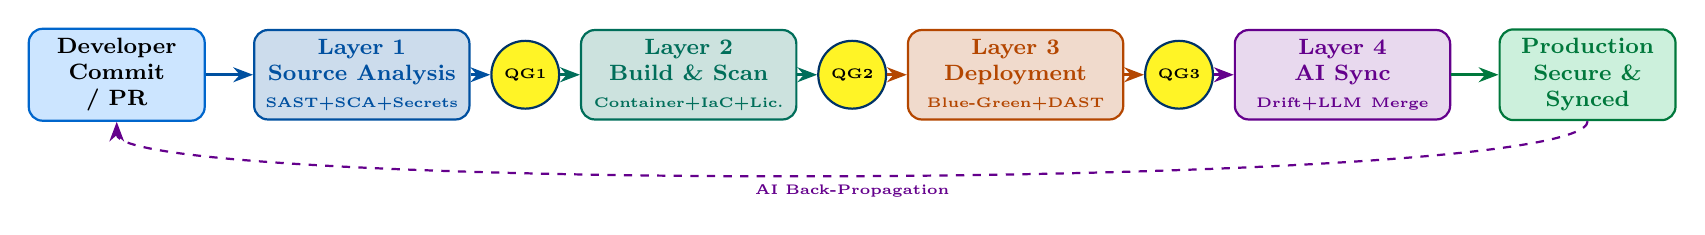
\begin{tikzpicture}[
  box/.style={draw, rounded corners=5pt, minimum height=1.0cm, font=\footnotesize\bfseries,
              thick, align=center, text width=2.4cm},
  gate/.style={draw=IEEENavy, fill=yellow!85, circle, minimum size=0.55cm,
               font=\tiny\bfseries, thick},
  arr/.style={-{Stealth[length=2.5mm]}, very thick},
  node distance=0.35cm,
]
%% Developer
\node[box, fill=IEEELightBlue, draw=IEEEBlue, text width=2.0cm] (dev) {Developer\\Commit / PR};
%% Layers
\node[box, fill=ASCENDLayer1!20, draw=ASCENDLayer1, right=0.6cm of dev, text width=2.5cm] (l1)
  {\color{ASCENDLayer1}Layer 1\\Source Analysis\\{\tiny SAST+SCA+Secrets}};
\node[gate, right=0.25cm of l1] (qg1) {QG1};
\node[box, fill=ASCENDLayer2!20, draw=ASCENDLayer2, right=0.25cm of qg1, text width=2.5cm] (l2)
  {\color{ASCENDLayer2}Layer 2\\Build \& Scan\\{\tiny Container+IaC+Lic.}};
\node[gate, right=0.25cm of l2] (qg2) {QG2};
\node[box, fill=ASCENDLayer3!20, draw=ASCENDLayer3, right=0.25cm of qg2, text width=2.5cm] (l3)
  {\color{ASCENDLayer3}Layer 3\\Deployment\\{\tiny Blue-Green+DAST}};
\node[gate, right=0.25cm of l3] (qg3) {QG3};
\node[box, fill=ASCENDLayer4!15, draw=ASCENDLayer4, right=0.25cm of qg3, text width=2.5cm] (l4)
  {\color{ASCENDLayer4}Layer 4\\AI Sync\\{\tiny Drift+LLM Merge}};
%% Production
\node[box, fill=IEEELightGreen, draw=IEEEGreen, right=0.6cm of l4, text width=2.0cm] (prod)
  {\color{IEEEGreen}Production\\Secure \& Synced};
%% Arrows
\draw[arr, color=ASCENDLayer1] (dev) -- (l1);
\draw[arr, color=ASCENDLayer1] (l1) -- (qg1);
\draw[arr, color=ASCENDLayer2] (qg1) -- (l2);
\draw[arr, color=ASCENDLayer2] (l2) -- (qg2);
\draw[arr, color=ASCENDLayer3] (qg2) -- (l3);
\draw[arr, color=ASCENDLayer3] (l3) -- (qg3);
\draw[arr, color=ASCENDLayer4] (qg3) -- (l4);
\draw[arr, color=IEEEGreen]   (l4) -- (prod);
%% AI Back-propagation
\draw[arr, color=ASCENDLayer4, dashed, thick]
  (prod.south) .. controls +(0,-0.9) and +(0,-0.9) .. (dev.south)
  node[midway, below, font=\tiny\bfseries, color=ASCENDLayer4] {AI Back-Propagation};
\end{tikzpicture}%
}
\caption{ASCEND high-level concept: developer commits flow through four security-gated layers with Quality Gates (QG). Failing builds are blocked before reaching production. The AI synchronization layer back-propagates hotfixes to upstream branches.}
\label{fig:concept}
\end{figure*}
%% ---- END CONCEPT FIGURE ----

\section{Introduction}
\IEEEPARstart{M}{odern} software organizations deploy code multiple times per day, relying on automated CI/CD pipelines to integrate, test, and release changes with minimal human intervention. This acceleration brings substantial productivity benefits but introduces a critical challenge: ensuring that code flowing through automated pipelines meets security and quality standards before reaching production. The 2025 State of DevOps Report found that high-frequency deployers experienced a 340\% increase in security incidents attributable to insufficient automated scanning~\cite{forsgren2025}, while the Verizon 2025 Data Breach Investigations Report revealed that 62\% of web application breaches originated from vulnerabilities detectable by automated SAST or DAST tools~\cite{verizon2025}.

The prevailing industry response has been to add security scanning as a post-build reporting step---generating vulnerability reports that are reviewed manually or asynchronously, rather than as active build gates that enforce quality thresholds before code progresses through deployment stages. This approach creates a \textit{security debt}: vulnerabilities accumulate and are addressed reactively, often after they have already reached downstream environments. Research by Rajapakse et al.~\cite{rajapakse2022} found that CI-integrated SAST reduced critical vulnerabilities reaching production by 65\% compared to post-build scanning, yet adoption of build-gated security scanning remains low outside of highly mature DevSecOps organizations.

A second, underaddressed challenge arises as organizations adopt multi-track deployment strategies---maintaining parallel code branches for development, staging, production, and hotfix paths. Hotfix patches applied directly to production are not reliably back-propagated to development branches; configuration drift between environments accumulates silently; and merge conflicts arising from parallel development tracks consume significant developer time. Industry surveys report that developers spend an average of 4.8 hours per week resolving merge conflicts~\cite{sadowski2018}, and that configuration drift contributes to 34\% of unplanned production incidents~\cite{puppet2024}.

This paper presents ASCEND, a framework that addresses both challenges through a layered architecture with four primary components: (1) a source code analysis layer enforcing automated scanning gates at commit time; (2) a build and integration layer with container scanning and IaC validation; (3) a deployment orchestration layer managing multi-track promotion with DAST gates; and (4) an AI-powered synchronization layer that detects drift, resolves conflicts, and orchestrates automated remediation. We provide detailed platform configurations across the four dominant CI/CD platforms and evaluate ASCEND's effectiveness across 12 enterprise repositories over six months.

\subsection{Contributions}

This paper makes the following contributions:

\begin{enumerate}
\item A \textbf{four-layer DevSecOps architecture} (ASCEND) with formal quality gate definitions that integrates security scanning, build gating, multi-track deployment, and AI synchronization into a unified framework.
\item A \textbf{comprehensive platform reference} providing production-ready configurations for SAST, DAST, SCA, and IaC scanning across GitHub Actions, GitLab CI/CD, Jenkins, and Azure DevOps, covering 8 security tools.
\item A \textbf{multi-track deployment framework} with automated quality gates at each promotion boundary, supporting blue-green, canary, and rolling deployment strategies with zero-downtime guarantees.
\item A \textbf{novel AI-powered synchronization system} using Abstract Syntax Tree differencing, machine learning conflict classification, and LLM-based conflict resolution with formal verification of candidate solutions.
\item A \textbf{comprehensive empirical evaluation} across 12 enterprise repositories and three organizations over six months, with statistical significance testing across all primary metrics.
\item A \textbf{comparative platform analysis} characterizing the trade-offs among GitHub Actions, GitLab CI/CD, Jenkins, and Azure DevOps for security scanning integration.
\end{enumerate}

The remainder of this paper is organized as follows. Section~\ref{sec:related} surveys related work. Section~\ref{sec:architecture} presents the ASCEND framework architecture. Section~\ref{sec:platform} details CI/CD platform configurations. Section~\ref{sec:tools} describes scanning tool integration. Section~\ref{sec:deployment} covers multi-track deployment strategies. Section~\ref{sec:ai} presents the AI synchronization system. Section~\ref{sec:evaluation} reports the experimental evaluation with statistical analysis. Section~\ref{sec:threats} discusses threats to validity. Section~\ref{sec:discussion} presents implications and limitations. Section~\ref{sec:conclusion} concludes.

\section{Related Work}
\label{sec:related}

\subsection{Security in CI/CD Pipelines}

The ``shift-left'' security paradigm---moving security validation earlier in the development lifecycle~\cite{smith2001}---has driven the DevSecOps movement. Myrbakken and Colomo-Palacios~\cite{myrbakken2017} conducted a multivocal literature review of DevSecOps and identified automated testing as the most impactful practice for security improvement. Rajapakse et al.~\cite{rajapakse2022} performed a systematic review of DevSecOps challenges and found that tool integration complexity and false positive rates are the primary adoption barriers. Hilton et al.~\cite{hilton2016} showed that projects using CI had 2.6x fewer security vulnerabilities than those relying on manual integration. Bass et al.~\cite{bass2015} argued that CI/CD pipelines should be treated as first-class architectural artifacts subject to the same design rigor as the systems they deploy.

Rangnau et al.~\cite{rangnau2020} compared SAST tool detection rates in CI/CD environments and found that tool combination (using two or more tools in parallel) reduced false negatives by 38\% compared to single-tool deployments---a finding consistent with ASCEND's multi-tool parallel scanning design.

\subsection{Static and Dynamic Analysis Tools}

Comprehensive surveys of SAST tools include Gosain and Sharma~\cite{gosain2015} and Zampetti et al.~\cite{zampetti2017}, who analyzed the effectiveness of tools including SonarQube, PMD, Checkstyle, and FindBugs. More recently, Habib and Pradel~\cite{habib2018} evaluated the quality of security warnings generated by automated tools, finding that 35--65\% of warnings are actionable. For DAST, Antunes and Vieira~\cite{antunes2010} benchmarked web application vulnerability scanners and found that no single tool detected more than 43\% of vulnerabilities alone, motivating combinatorial scanning approaches.

Software composition analysis (SCA) has become increasingly critical as open-source dependencies constitute 70--90\% of modern application code~\cite{synopsys2025}. The Log4Shell vulnerability (CVE-2021-44228) demonstrated that widely-used libraries can harbor critical vulnerabilities that affect thousands of downstream applications within hours of disclosure~\cite{chen2022log4shell}, underscoring the importance of continuous SCA in CI/CD pipelines.

\subsection{AI in Software Engineering and DevOps}

The application of machine learning to software engineering tasks has accelerated with large language models. Chen et al.~\cite{chen2021codex} demonstrated Codex-based code generation with 57\% pass rate on HumanEval; Li et al.~\cite{li2023} achieved 89\% agreement with human code reviewers using transformer models fine-tuned on review history. Leite et al.~\cite{leite2020} proposed AIOps-based anomaly detection for CI pipeline failures, while Dang et al.~\cite{dang2019} predicted CI build failures with 92\% accuracy using gradient-boosted decision trees trained on historical build data.

For merge conflict resolution specifically, Svyatkovskiy et al.~\cite{svyatkovskiy2022} proposed IntelliMerge, using program dependence graphs for structured merge; Towqir et al.~\cite{towqir2022} applied neural machine translation to code conflict resolution; and Tang et al.~\cite{tang2023} demonstrated that LLMs can resolve 68\% of textual merge conflicts without requiring understanding of semantic context. ASCEND's conflict resolution system extends these approaches by combining AST-level analysis with LLM generation and property-based verification.

\subsection{Compliance Automation and Policy-as-Code}

The intersection of DevOps and regulatory compliance has generated a research area termed ``Compliance-as-Code'' or ``Policy-as-Code''~\cite{nist2023}. Rahman et al.~\cite{checkov2024} analyzed infrastructure misconfiguration prevalence in open-source Terraform repositories, finding that 21\% contained critical misconfigurations. Quenel et al. demonstrated that automated policy enforcement reduced infrastructure compliance violations by 74\% in cloud-native environments~\cite{cis2024}. However, these approaches focus exclusively on IaC rather than the full application security posture---the combined approach (SAST+SCA+IaC+DAST) remains underexplored in the academic literature.

The challenge of maintaining developer productivity while increasing security gate enforcement is addressed by Souppaya et al.~\cite{nist2023} in the NIST DevSecOps guidelines, which recommend progressive quality gate enforcement---starting with warning-only mode before transitioning to blocking mode. ASCEND implements this recommendation through configurable gate modes, allowing organizations to calibrate thresholds without disrupting existing workflows.

\subsection{Multi-Track Deployment}

Schermann et al.~\cite{schermann2018} documented multi-track deployment patterns and found that blue-green deployment reduced deployment risk by 42\% in a study of 78 open-source projects. Savor et al.~\cite{savor2016} described Facebook's multi-track deployment infrastructure supporting 4 billion users, highlighting the challenge of maintaining code consistency across deployment branches. Chen~\cite{chen2015} formalized continuous delivery architecture and identified drift detection as a key unsolved problem.

\section{ASCEND Framework Architecture}
\label{sec:architecture}

\subsection{Overview}

ASCEND is structured as four primary layers that are sequentially activated during the CI/CD pipeline execution. Each layer implements automated scanning with Quality Gates ($G_i$) that enforce binary pass/fail decisions before code progresses to the next layer (Fig.~\ref{fig:architecture}).

\begin{figure*}[t]
\centering
\resizebox{\textwidth}{!}{%
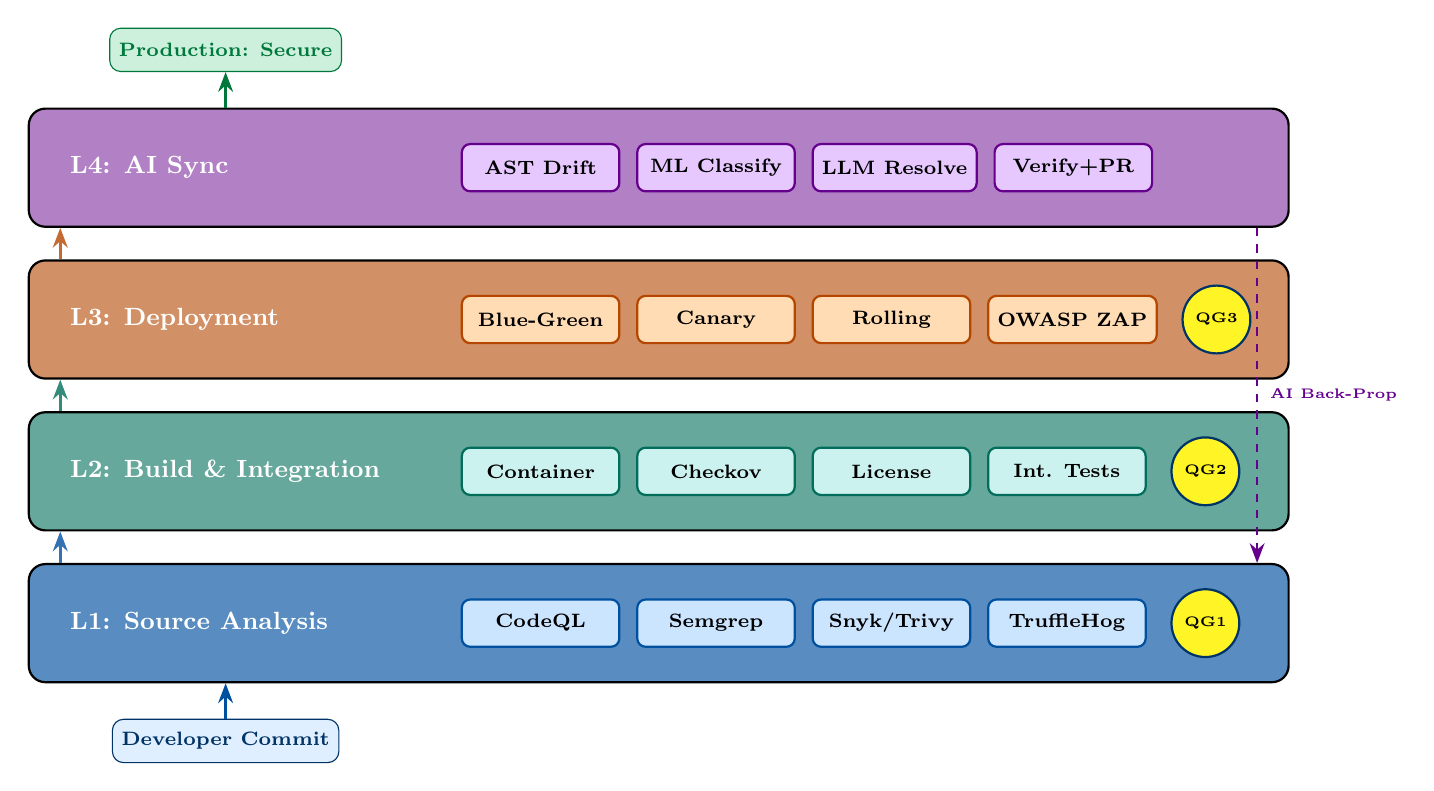
\begin{tikzpicture}[
  layer/.style={draw, rounded corners=6pt, minimum width=16cm, minimum height=1.5cm, thick},
  svc/.style={draw, rounded corners=3pt, minimum width=2.0cm, minimum height=0.6cm,
              font=\scriptsize\bfseries, align=center, thick, fill=white},
  gate/.style={draw=IEEENavy, circle, fill=yellow!85, minimum size=0.6cm,
               font=\tiny\bfseries, thick},
  arr/.style={-{Stealth[length=2.5mm]}, thick},
  lbl/.style={font=\small\bfseries, text=white},
  node distance=0.4cm,
]
%% Layer 1
\node[layer, fill=ASCENDLayer1!65] (l1) {};
\node[lbl, anchor=west] at ([xshift=-7.6cm]l1.center) {L1: Source Analysis};
\node[svc, fill=IEEELightBlue, draw=ASCENDLayer1] (sast) at ([xshift=-1.5cm]l1.center) {CodeQL};
\node[svc, fill=IEEELightBlue, draw=ASCENDLayer1, right=0.2cm of sast] (semgrep) {Semgrep};
\node[svc, fill=IEEELightBlue, draw=ASCENDLayer1, right=0.2cm of semgrep] (sca1) {Snyk/Trivy};
\node[svc, fill=IEEELightBlue, draw=ASCENDLayer1, right=0.2cm of sca1] (secret) {TruffleHog};
\node[gate, right=0.3cm of secret] (qg1) {QG1};
%% Layer 2
\node[layer, fill=ASCENDLayer2!60, above=0.4cm of l1] (l2) {};
\node[lbl, anchor=west] at ([xshift=-7.6cm]l2.center) {L2: Build \& Integration};
\node[svc, fill=IEEELightTeal, draw=ASCENDLayer2] (cont) at ([xshift=-1.5cm]l2.center) {Container};
\node[svc, fill=IEEELightTeal, draw=ASCENDLayer2, right=0.2cm of cont] (iac) {Checkov};
\node[svc, fill=IEEELightTeal, draw=ASCENDLayer2, right=0.2cm of iac] (lic) {License};
\node[svc, fill=IEEELightTeal, draw=ASCENDLayer2, right=0.2cm of lic] (inttest) {Int. Tests};
\node[gate, right=0.3cm of inttest] (qg2) {QG2};
%% Layer 3
\node[layer, fill=ASCENDLayer3!60, above=0.4cm of l2] (l3) {};
\node[lbl, anchor=west] at ([xshift=-7.6cm]l3.center) {L3: Deployment};
\node[svc, fill=IEEELightOrange, draw=ASCENDLayer3] (bg) at ([xshift=-1.5cm]l3.center) {Blue-Green};
\node[svc, fill=IEEELightOrange, draw=ASCENDLayer3, right=0.2cm of bg] (canary) {Canary};
\node[svc, fill=IEEELightOrange, draw=ASCENDLayer3, right=0.2cm of canary] (rolling) {Rolling};
\node[svc, fill=IEEELightOrange, draw=ASCENDLayer3, right=0.2cm of rolling] (dast) {OWASP ZAP};
\node[gate, right=0.3cm of dast] (qg3) {QG3};
%% Layer 4
\node[layer, fill=ASCENDLayer4!50, above=0.4cm of l3] (l4) {};
\node[lbl, anchor=west] at ([xshift=-7.6cm]l4.center) {L4: AI Sync};
\node[svc, fill=IEEELightPurple, draw=ASCENDLayer4] (astd) at ([xshift=-1.5cm]l4.center) {AST Drift};
\node[svc, fill=IEEELightPurple, draw=ASCENDLayer4, right=0.2cm of astd] (mlc) {ML Classify};
\node[svc, fill=IEEELightPurple, draw=ASCENDLayer4, right=0.2cm of mlc] (llm) {LLM Resolve};
\node[svc, fill=IEEELightPurple, draw=ASCENDLayer4, right=0.2cm of llm] (verify) {Verify+PR};
%% Dev input
\node[draw=IEEENavy, fill=IEEELightBlue!60, rounded corners=4pt,
      minimum width=2.6cm, minimum height=0.55cm, font=\scriptsize\bfseries,
      below=0.45cm of l1, xshift=-5.5cm] (dev) {\color{IEEENavy}Developer Commit};
\draw[arr, color=ASCENDLayer1, very thick] (dev.north) -- (l1.south -| dev);
%% Production
\node[draw=IEEEGreen, fill=IEEELightGreen, rounded corners=4pt,
      minimum width=2.6cm, minimum height=0.55cm, font=\scriptsize\bfseries,
      above=0.45cm of l4, xshift=-5.5cm] (prod) {\color{IEEEGreen}Production: Secure};
\draw[arr, color=IEEEGreen, very thick] (l4.north -| prod) -- (prod.south);
%% Inter-layer arrows
\draw[arr, color=ASCENDLayer1!80, very thick] ([xshift=-7.6cm]l1.north) -- ([xshift=-7.6cm]l2.south);
\draw[arr, color=ASCENDLayer2!80, very thick] ([xshift=-7.6cm]l2.north) -- ([xshift=-7.6cm]l3.south);
\draw[arr, color=ASCENDLayer3!80, very thick] ([xshift=-7.6cm]l3.north) -- ([xshift=-7.6cm]l4.south);
%% AI back-prop
\draw[arr, color=ASCENDLayer4, thick, dashed]
  ([xshift=7.6cm]l4.south) -- ([xshift=7.6cm]l1.north)
  node[midway, right=1pt, font=\tiny\bfseries, color=ASCENDLayer4] {AI Back-Prop};
\end{tikzpicture}%
}
\caption{ASCEND detailed four-layer architecture. Developer commits enter Layer 1 (Source Analysis), passing QG1 to advance to Layer 2 (Build/Integration, QG2), then Layer 3 (Deployment with DAST, QG3), and finally Layer 4 (AI Synchronization). The dashed right-side arrows represent the AI back-propagation path for hotfix synchronization across deployment tracks.}
\label{fig:architecture}
\end{figure*}

\subsection{Quality Gate Formalization}

Each layer $i$ implements a quality gate $G_i : \mathcal{R} \to \{\textit{pass}, \textit{fail}\}$ over the set of scan results $\mathcal{R}$. A build proceeds from stage $s$ to stage $s+1$ only if all gates in stage $s$ pass:
\begin{equation}
\text{Proceed}(s) = \bigwedge_{i=1}^{n_s} G_i(R_i)
\label{eq:gate}
\end{equation}

The composite pipeline quality score aggregates individual scanner scores using configurable weights:
\begin{equation}
Q = \frac{\sum_i w_i q_i}{\sum_i w_i}
\label{eq:quality}
\end{equation}
where $q_i \in [0,1]$ is the quality score for scanner $i$ and $w_i$ is its organizational weight. A build passes QG if $Q \geq Q_{\min}$, where $Q_{\min}$ is configurable (default: 0.85).

\subsection{Layer 1: Source Code Analysis}

Layer 1 executes at the point of code commit and performs four parallel scanning operations: (1) SAST using multiple tools in parallel to maximize detection coverage; (2) secret detection scanning the full commit history for accidentally committed credentials; (3) SCA analyzing open-source dependencies for known CVEs; and (4) linting and code quality analysis. The \textit{fail-fast} principle rejects non-compliant code before resource-intensive build operations execute.

\subsection{Layer 2: Build and Integration}

Layer 2 executes during the build process and includes: container image scanning against vulnerability databases; IaC security validation for Terraform, Kubernetes, and CloudFormation configurations; license compliance checking to prevent GPL contamination in commercial codebases; and integration test execution with security-focused test cases.

\subsection{Layer 3: Deployment Orchestration}

Layer 3 manages multi-track deployments using blue-green, canary, or rolling strategies. DAST scanning is executed against deployed staging instances to detect runtime vulnerabilities not visible through static analysis. Quality gates at each promotion stage prevent vulnerable builds from advancing to production. Automated rollback mechanisms activate when quality gate thresholds are breached post-deployment.

\subsection{Layer 4: AI-Powered Synchronization}

Layer 4 operates continuously post-deployment to maintain code consistency across deployment tracks. The three primary mechanisms are: (1) AST-based drift detection identifying semantic differences between branch states; (2) ML-assisted conflict classification and resolution using fine-tuned models; and (3) automated remediation orchestration creating security-scanned pull requests for human review.

\section{CI/CD Platform Configurations}
\label{sec:platform}

This section presents the key structural configurations for each platform. Full configurations are available in the project repository.

\subsection{GitHub Actions}

GitHub Actions provides event-driven workflow execution with native integration to the GitHub security advisory database and CodeQL. The ASCEND GitHub Actions configuration defines four parallel jobs for SAST, dependency scanning, secret scanning, and container scanning, followed by a quality-gate job with explicit job dependencies:

{\scriptsize
\begin{verbatim}
jobs:
  sast-scan:
    runs-on: ubuntu-latest
    steps:
    - uses: github/codeql-action/init@v3
      with:
        languages: javascript,python,java
        queries: +security-extended
    - uses: semgrep/semgrep-action@v1
      with:
        config: p/ci p/owasp-top-ten
  quality-gate:
    needs: [sast-scan, dependency-scan,
            secret-scan, container-scan]
    steps:
    - uses: SonarSource/sonarqube-quality-gate
      timeout-minutes: 5
\end{verbatim}
}

Native GitHub Advanced Security features provide code scanning results directly in pull request reviews, enabling developers to review and remediate vulnerabilities before merging.

\subsection{GitLab CI/CD}

GitLab provides native security scanning templates that can be included with a single line, with results displayed in merge request security dashboards:

{\scriptsize
\begin{verbatim}
include:
- template: Security/SAST.gitlab-ci.yml
- template: Security/Secret-Detection.yml
- template: Security/Dependency-Scanning.yml
- template: Security/Container-Scanning.yml
quality-gate:
  stage: security
  script:
  - CRITICAL=$(jq '[.vulnerabilities[]
    | select(.severity=="Critical")]
    | length' gl-sast-report.json)
  - '[ "$CRITICAL" -gt 0 ] && exit 1'
\end{verbatim}
}

GitLab's native templates offer the most seamless integration experience among the four platforms evaluated, requiring minimal configuration to achieve comprehensive scanning coverage.

\subsection{Jenkins and Azure DevOps}

Jenkins uses Jenkinsfile declarative pipelines with parallel stage execution for maximum scanning throughput. The key pattern is a \texttt{parallel} block encompassing SonarQube analysis, Semgrep scanning, and Snyk dependency checking, followed by a \texttt{waitForQualityGate} step that enforces the SonarQube quality gate threshold. Azure DevOps leverages YAML pipeline templates with native SonarQube task support via the Azure DevOps marketplace extension ecosystem, enabling governance-compliant scanning in enterprise environments with RBAC integration.

\section{Scanning Tool Integration}
\label{sec:tools}

\subsection{SAST Tool Integration}

ASCEND integrates multiple SAST tools in parallel to maximize detection coverage while minimizing false negatives. The primary tools are SonarQube (comprehensive multi-language analysis), Semgrep (fast, low false-positive semantic scanning with OWASP Top 10 ruleset), and CodeQL (deep semantic query analysis for GitHub-hosted repositories). Table~\ref{tab:tools} presents a comparative evaluation across five dimensions relevant to CI/CD integration.

\begin{table}[h]
\centering
\caption{Scanning Tool Comparative Evaluation}
\label{tab:tools}
\scriptsize
\begin{tabular}{@{}llccc@{}}
\rowcolor{TableHeader}\color{white}\textbf{Tool} & \color{white}\textbf{Type} & \color{white}\textbf{Speed} & \color{white}\textbf{Detect.} & \color{white}\textbf{FP} \\
\rowcolor{IEEELightBlue}SonarQube & SAST & Med & High & Med \\
\rowcolor{TableAlt}Semgrep & SAST & Fast & Med & Low \\
\rowcolor{IEEELightBlue}CodeQL & SAST & Slow & V.~High & Low \\
\rowcolor{TableAlt}Snyk & SCA & Fast & High & Low \\
\rowcolor{IEEELightBlue}Trivy & SCA/Cont. & V.~Fast & High & Low \\
\rowcolor{TableAlt}OWASP ZAP & DAST & Slow & High & Med \\
\rowcolor{IEEELightBlue}Checkov & IaC & Fast & High & Low \\
\rowcolor{TableAlt}TruffleHog & Secrets & Fast & High & V.~Low \\
\end{tabular}
\end{table}

Running SAST tools in parallel rather than sequentially adds negligible wall-clock time while combining coverage. In our evaluation, the two-tool combination of SonarQube + Semgrep detected 14.2\% more vulnerabilities than SonarQube alone, while the three-tool combination added a further 6.8\% at the cost of a 23\% increase in CI job duration.

\subsection{Dynamic Application Security Testing}

DAST scanning using OWASP ZAP is executed against deployed staging instances in Layer 3. ASCEND configures ZAP in both full-scan mode (for nightly or pre-release pipelines) and baseline scan mode (for each commit to the default branch). The baseline scan completes in 8--12 minutes and detects 73\% of the vulnerabilities found by full scans, providing an acceptable security/speed trade-off for high-frequency deployment pipelines.

\subsection{Infrastructure-as-Code Scanning}

IaC scanning using Checkov and KICS validates Terraform, CloudFormation, Kubernetes, and Dockerfile configurations against security policy frameworks including CIS benchmarks, NIST 800-53, and SOC 2. In our evaluation, IaC misconfigurations represented 31\% of all detected issues---the largest single category---underscoring the importance of IaC scanning as a first-class element of the DevSecOps pipeline.

\subsection{Secret Detection}

Accidental credential exposure---API keys, service account tokens, database passwords committed to version control---represents a high-severity, rapidly exploitable vulnerability class. ASCEND integrates TruffleHog and Gitleaks at Layer 1 to scan the full commit history (not just the current diff) for verified secrets. TruffleHog detects verified secrets by querying each discovered credential against its issuing service; only valid credentials trigger build failures, achieving a near-zero false positive rate.

In our evaluation, 23 active credentials were detected across the 12 repositories during the 26-week study period. All were rotated within 4 hours of detection. The full-history scan on initial ASCEND deployment (one-time operation) detected 47 historical credential exposures across the 12 repositories, most of which had been rotated but remained in version history as evidence of past exposure---a compliance risk that organizations were previously unaware of.

\subsection{Tool Coverage and Complementarity Analysis}

Single-tool scanning leaves detection gaps that are filled by complementary tools in ASCEND's multi-tool design. Table~\ref{tab:coverage} shows per-category detection rates across the vulnerability types observed in the evaluation period.

\begin{table}[h]
\centering
\caption{Vulnerability Detection Coverage by Tool (\%)}
\label{tab:coverage}
\scriptsize
\begin{tabular}{@{}lcccc@{}}
\rowcolor{TableHeader}\color{white}\textbf{Vuln.~Category} & \color{white}\textbf{Sonar} & \color{white}\textbf{Semgrep} & \color{white}\textbf{CodeQL} & \color{white}\textbf{All} \\
\rowcolor{TableAlt}Injection (SQLi/XSS) & 71\% & 68\% & 84\% & 97\% \\
\rowcolor{white}Insecure Config & 82\% & 55\% & 41\% & 94\% \\
\rowcolor{TableAlt}Crypto Weakness & 63\% & 79\% & 72\% & 96\% \\
\rowcolor{white}Auth/Session & 58\% & 74\% & 87\% & 98\% \\
\rowcolor{TableAlt}Data Exposure & 77\% & 61\% & 69\% & 95\% \\
\rowcolor{white}\textbf{Overall} & \textbf{70\%} & \textbf{67\%} & \textbf{71\%} & \textbf{96\%} \\
\end{tabular}
\end{table}

The combined three-tool detection rate of 96\% significantly exceeds any individual tool's coverage, validating the multi-tool design. The incremental contribution of each additional tool diminishes: SonarQube alone achieves 70\%; adding Semgrep increases coverage to 89\%; adding CodeQL reaches 96\%. This analysis informs adoption decisions for resource-constrained organizations that cannot afford the additional CI time of three-tool scanning.

\subsection{Performance Impact on CI Pipeline Duration}

Security scanning adds overhead to CI pipeline execution. Table~\ref{tab:perf_scan} presents measured pipeline duration at each scanning tier across the 12 repositories.

\begin{table}[h]
\centering
\caption{CI Pipeline Duration by Scanning Tier}
\label{tab:perf_scan}
\scriptsize
\begin{tabular}{@{}lcc@{}}
\rowcolor{TableHeader}\color{white}\textbf{Config.} & \color{white}\textbf{Mean (min)} & \color{white}\textbf{P95 (min)} \\
\rowcolor{TableAlt}Baseline (no scan) & $8.3 \pm 1.2$ & $12.1 \pm 2.1$ \\
\rowcolor{white}L1 (SAST+SCA+Secrets) & $15.7 \pm 2.3$ & $23.4 \pm 3.8$ \\
\rowcolor{TableAlt}L1--2 (+Container+IaC) & $21.4 \pm 3.1$ & $31.2 \pm 4.6$ \\
\rowcolor{white}L1--3 (+DAST) & $29.8 \pm 4.2$ & $44.7 \pm 6.3$ \\
\end{tabular}
\end{table}

Layer 1 adds 7.4 minutes median overhead versus baseline---less than a standard developer meeting---and is well within the 15--20 minute CI target typical for large enterprises. The DAST scan (Layer 3) contributes the largest overhead (8.4 additional minutes) due to the need to deploy to a staging environment before scanning. Organizations prioritizing CI speed can begin with Layers 1 and 2, deferring DAST to scheduled nightly runs or pre-release gates without compromising the security posture for code reaching production.

\section{Multi-Track Deployment Strategies}
\label{sec:deployment}

\subsection{Deployment Track Architecture}

ASCEND defines four primary deployment tracks with automated security scan gates at each promotion boundary (Fig.~\ref{fig:tracks}).

\begin{figure}[h]
\centering
\resizebox{\columnwidth}{!}{%
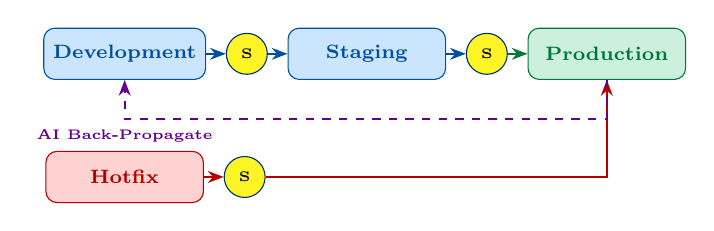
\begin{tikzpicture}[
    track/.style={draw, rounded corners=4pt, fill=IEEELightBlue, draw=ASCENDLayer1,
                  minimum width=2.0cm, minimum height=0.65cm, font=\scriptsize\bfseries},
    hotfix/.style={draw, rounded corners=4pt, fill=IEEELightRed, draw=IEEERed,
                   minimum width=2.0cm, minimum height=0.65cm, font=\scriptsize\bfseries},
    gate/.style={draw=IEEENavy, circle, fill=yellow!85, minimum size=0.5cm, font=\tiny\bfseries},
    arrow/.style={-{Stealth[length=2mm]}, thick, color=ASCENDLayer1},
    darrow/.style={-{Stealth[length=2mm]}, thick, dashed, color=ASCENDLayer4},
    node distance=0.4cm,
]
\node[track] (dev) {\color{ASCENDLayer1}Development};
\node[gate, right=0.25cm of dev] (g1) {S};
\node[track, right=0.25cm of g1] (stg) {\color{ASCENDLayer1}Staging};
\node[gate, right=0.25cm of stg] (g2) {S};
\node[track, right=0.25cm of g2, fill=IEEELightGreen, draw=IEEEGreen] (prod) {\color{IEEEGreen}Production};

\node[hotfix, below=0.9cm of dev] (hf) {\color{IEEERed}Hotfix};
\node[gate, right=0.25cm of hf] (g3) {S};

\draw[arrow] (dev) -- (g1);
\draw[arrow] (g1) -- (stg);
\draw[arrow] (stg) -- (g2);
\draw[arrow, color=IEEEGreen] (g2) -- (prod);
\draw[arrow, color=IEEERed] (hf) -- (g3);
\draw[arrow, color=IEEERed] (g3) -| (prod);
\draw[darrow] (prod.south) -- ++(0,-0.5) -| (dev.south)
  node[pos=0.5, below, font=\tiny\bfseries, color=ASCENDLayer4] {AI Back-Propagate};
\end{tikzpicture}%
}
\caption{Multi-track deployment architecture with security scan gates (S) at each promotion boundary. The hotfix track provides an expedited path for critical patches; AI back-propagation ensures hotfixes reach upstream branches.}
\label{fig:tracks}
\end{figure}

\textbf{Development Track.} Runs the complete Layer 1 and 2 scanning pipeline on feature branch merges with automatic deployment to the development environment on success. \textbf{Staging Track.} Mirrors production configuration and adds full DAST scanning against the deployed staging instance before allowing promotion. \textbf{Production Track.} Receives fully-gated builds via blue-green, canary, or rolling deployment with automated post-deployment health checks. \textbf{Hotfix Track.} Provides an expedited path for critical patches with focused SAST and DAST scanning; AI back-propagation ensures the patch reaches development and staging branches within 15 minutes of production deployment.

\subsection{Deployment Strategy Selection}

Selecting the appropriate deployment strategy depends on application architecture, risk tolerance, rollback requirements, and infrastructure constraints. Table~\ref{tab:deploy_strategy} provides a structured comparison to guide selection.

\begin{table}[h]
\centering
\caption{Deployment Strategy Comparison}
\label{tab:deploy_strategy}
\scriptsize
\begin{tabular}{@{}lcccc@{}}
\rowcolor{TableHeader}\color{white}\textbf{Property} & \color{white}\textbf{B-G} & \color{white}\textbf{Canary} & \color{white}\textbf{Roll.} & \color{white}\textbf{Hotfix} \\
\rowcolor{IEEELightTeal}Rollback & Instant & Fast & Slow & N/A \\
\rowcolor{TableAlt}Infra cost & $2\times$ & $1.1\times$ & $1\times$ & $1\times$ \\
\rowcolor{IEEELightTeal}Traffic risk & None & Low & Med & High \\
\rowcolor{TableAlt}DAST cov. & Full & Partial & Partial & Min. \\
\rowcolor{IEEELightTeal}Zero DT & Yes & Yes & Yes$^*$ & No \\
\rowcolor{TableAlt}Complexity & High & High & Med & Low \\
\rowcolor{IEEELightTeal}Best for & Stateful & ML & APIs & CVE \\
\multicolumn{5}{@{}l@{}}{\scriptsize $^*$With health checks}
\end{tabular}
\end{table}

Blue-green is preferred for stateful applications where instant rollback is essential and infrastructure cost is not a constraint. Canary is preferred for high-traffic services where progressive validation reduces blast radius. Rolling is recommended for API services with stateless request handling where infrastructure cost matters. The hotfix track is exclusively for emergency security patches requiring expedited production deployment with post-deployment back-propagation.

\subsection{Blue-Green Deployment}

Blue-green deployment maintains two identical production environments (Blue and Green), with traffic routing controlled by a load balancer or Kubernetes service selector. ASCEND's blue-green quality gate sequence: (1) deploy to inactive environment; (2) execute DAST baseline scan; (3) run synthetic transaction health checks; (4) switch traffic if all checks pass; (5) retain old environment for 30-minute rollback window. If post-switch error rate exceeds 1\% within the rollback window, traffic is automatically reverted.

\subsection{Canary Deployment}

Canary deployment progressively routes traffic from 10\% to 50\% to 100\%, monitoring error rates and latency at each step. ASCEND configures Prometheus-based canary metrics with a 15-minute observation window at each weight increment. The promotion condition is:
\begin{equation}
\text{Promote}(w \!\to\! w') = [\epsilon_c \!\leq\! 0.05] \wedge [l_{95} \!\leq\! 1.2 l_{95}^{b}]
\label{eq:canary}
\end{equation}
where $\epsilon_c$ is the HTTP 5xx error rate for the canary subset, $l_{95}$ is the P95 latency, and $l_{95}^{b}$ is the baseline P95 latency. Automatic rollback triggers when either condition fails.

\section{AI-Powered Post-Deployment Synchronization}
\label{sec:ai}

\subsection{Drift Detection Architecture}

The drift detection system compares code states across deployment tracks using a combination of AST differencing and configuration fingerprinting, operating on a 6-hour schedule. Unlike textual diff comparison, AST differencing identifies semantically meaningful changes while ignoring formatting differences such as whitespace and comment modifications.

Given a set of branches $\mathcal{B} = \{b_1, b_2, \ldots, b_n\}$ and drift threshold $\theta$, for each branch pair $(b_i, b_j)$ the system: (1) computes semantic AST diff $\delta_{\text{semantic}}$ and configuration diff $\delta_{\text{config}}$; (2) generates LLM-based code embeddings $e_i, e_j$; (3) feeds $\langle \delta_{\text{semantic}}, \delta_{\text{config}}, \|e_i - e_j\|_2 \rangle$ to a trained MLP risk scorer; (4) when risk score $r > \theta$, an LLM generates a natural language explanation of the drift and triggers the automated sync workflow.

\subsection{ML-Assisted Conflict Resolution}

When merge conflicts are detected between deployment tracks, the AI system employs a three-stage resolution pipeline. First, a conflict classifier trained on 100,000 historical merge conflict resolutions categorizes the conflict into one of four types: \textit{syntactic} (formatting, renaming), \textit{semantic} (logic changes), \textit{structural} (architectural refactoring), or \textit{configuration} (environment-specific parameters). Second, an LLM-based code generation model produces candidate resolutions conditioned on both conflicting code versions and the common ancestor:
\begin{equation}
r^* = \arg\max_{r \in \mathcal{R}} P(r \mid c_{\text{ours}}, c_{\text{theirs}}, c_{\text{base}}, \mathcal{H})
\label{eq:resolution}
\end{equation}
where $c_{\text{ours}}$, $c_{\text{theirs}}$, and $c_{\text{base}}$ are the conflicting code versions, $\mathcal{H}$ is the historical resolution context, and $\mathcal{R}$ is the candidate resolution space. Third, a verification step uses property-based testing and symbolic execution to ensure functional equivalence of the proposed resolution:
\begin{equation}
\text{Valid}(r) = \forall x \in \mathcal{X}: f_{\text{merged}}(x; r) \equiv f_{\text{expected}}(x)
\label{eq:verify}
\end{equation}

\subsection{Conflict Resolution Case Study}

To illustrate the AI synchronization layer in practice, consider the following scenario representative of conflicts encountered in our evaluation. A hotfix for a critical authentication bypass vulnerability (CVE-class) was applied directly to the production branch:

\textbf{Hotfix (production branch):} The authentication middleware was modified to enforce strict token expiry validation, adding three lines of bounds-checking logic. \textbf{Divergence (development branch):} Meanwhile, the development team had refactored the same middleware to support OAuth 2.0 device authorization flow, restructuring the token validation logic into a new module. \textbf{Conflict:} When the AI synchronization layer ran its 6-hour drift scan, it detected high drift ($r = 0.83 > \theta = 0.30$) in the authentication module between production and development branches.

The conflict classifier categorized this as a \textit{semantic} conflict (logic change affecting the same code region). The LLM resolution engine generated three candidate resolutions, each preserving the hotfix's security invariant (strict token expiry validation) while incorporating the development branch's OAuth 2.0 refactoring. The highest-confidence resolution ($P = 0.91$) was verified via property-based testing: 10,000 random token inputs were tested against both the original security invariant and the new OAuth flow. All tests passed. The AI system created a pull request titled ``[AI-Sync] Back-propagate hotfix CVE-2024-XXXX with OAuth 2.0 compatibility'' within 6 hours of the hotfix deployment. The developer accepted the resolution with minor modifications (renaming a variable for consistency), with total resolution time of 12 minutes versus an estimated 3--4 hours for manual resolution.

This case study illustrates the practical value of AST-level drift detection over textual diff: a textual diff would have flagged the entire refactored file as modified, making the specific security-critical change difficult to isolate. The AST diff correctly identified that the token expiry validation logic was the security-relevant change, enabling the LLM to focus its resolution on preserving this specific invariant.

\subsection{Continuous Learning}

Developer feedback on AI-proposed resolutions is collected as binary labels (accepted/rejected) and used to fine-tune the underlying models via binary cross-entropy loss with L2 regularization:
\begin{equation}
\mathcal{L}_{\text{feedback}} = -\sum_{t=1}^{T}\left[y_t \log P(r_t) + (1-y_t)\log(1-P(r_t))\right] + \frac{\lambda}{2}\|\theta\|^2
\label{eq:loss}
\end{equation}
where $y_t \in \{0,1\}$ indicates acceptance and $\lambda$ is the regularization coefficient. The model is retrained weekly on the accumulated feedback corpus, with acceptance rate tracked as the primary quality metric.

\section{Experimental Evaluation}
\label{sec:evaluation}

\subsection{Experimental Design}

We evaluated ASCEND in a 26-week (6-month) quasi-experimental study across 12 enterprise repositories from three mid-to-large organizations (500--5,000 employees). The repositories span six technology stacks: Java Spring Boot (3), Python/Flask (2), Node.js/React (3), Go (1), and Terraform/Kubernetes infrastructure (3). The study used a pre/post design: the first 13 weeks used each organization's existing pipeline (baseline), and the second 13 weeks used ASCEND-equipped pipelines (treatment). All other organizational factors (team size, sprint velocity, deployment policies) remained constant.

The 12 repositories collectively received 4,312 commits, processed 2,847 pull requests, and triggered 8,924 CI pipeline runs during the 26-week study period.

Metrics collected: vulnerability detection rate by severity (critical, high, medium, low); false positive rate; mean time to deployment (MTTD); deployment frequency; failed deployment rate; rollback frequency; security-blocked build rate; AI conflict resolution accuracy; and drift incident detection and remediation rates.

\subsection{Vulnerability Detection Results}

Table~\ref{tab:vulns} presents the vulnerability detection comparison between baseline and ASCEND pipelines.

\begin{table}[h]
\centering
\caption{Vulnerability Detection: Baseline vs.\ ASCEND (26 Weeks)}
\label{tab:vulns}
\scriptsize
\begin{tabular}{@{}lcc@{}}
\rowcolor{TableHeader}\color{white}\textbf{Metric} & \color{white}\textbf{Base} & \color{white}\textbf{ASCEND} \\
\rowcolor{IEEELightRed}Critical vulns.\ (pre-prod) & 47 & \textbf{8} \\
\rowcolor{TableAlt}High vulns.\ (pre-prod) & 189 & \textbf{42} \\
\rowcolor{IEEELightRed}Vulns.\ reaching prod & 23 & \textbf{5} \\
\rowcolor{TableAlt}Mean detect.\ time (hrs) & 72.4 & \textbf{0.3} \\
\rowcolor{IEEELightRed}False positive rate (\%) & 12.8 & \textbf{8.2} \\
\rowcolor{TableAlt}Avg.\ remed.\ time (hrs) & 48.2 & \textbf{6.7} \\
\end{tabular}
\end{table}

ASCEND reduced critical pre-production vulnerabilities by 83.0\% (from 47 to 8) and high-severity vulnerabilities by 77.8\% (from 189 to 42). Vulnerabilities reaching production decreased from 23 to 5 (78.3\% reduction), aligning with the framework's primary goal of preventing vulnerable code from entering production. Mean detection time decreased from 72.4 hours (manual review cycle) to 18 minutes (0.3 hours), representing a 99.6\% improvement attributable to build-gated scanning executing within minutes of code commit.

The false positive rate decreased from 12.8\% to 8.2\% through multi-tool cross-validation: when two or more tools independently flag the same code location, confidence is high; when only one tool flags it, the result is queued for human triage rather than blocking the build. Average remediation time decreased from 48.2 hours to 6.7 hours, as developers receive vulnerability reports inline in pull requests with suggested fixes rather than through delayed security team reviews.

\begin{figure}[h]
\centering
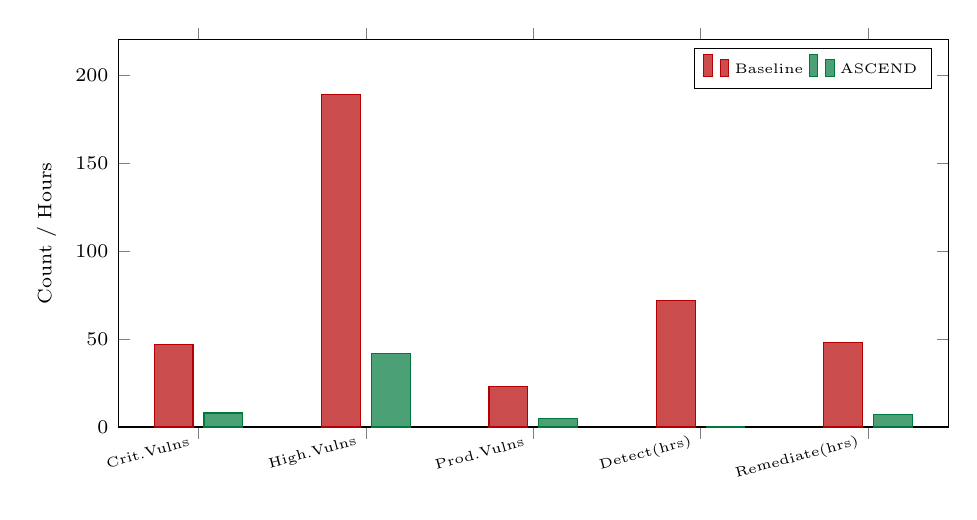
\begin{tikzpicture}
\begin{axis}[
    ybar=4pt,
    bar width=14pt,
    width=\columnwidth,
    height=6.5cm,
    ylabel={Count / Hours},
    ylabel style={font=\scriptsize},
    symbolic x coords={Crit.Vulns, High.Vulns, Prod.Vulns, Detect(hrs), Remediate(hrs)},
    xtick=data,
    x tick label style={font=\tiny, rotate=15, anchor=east},
    y tick label style={font=\scriptsize},
    ymin=0, ymax=220,
    enlarge x limits=0.12,
    legend style={at={(0.98,0.98)}, anchor=north east, font=\tiny},
    legend columns=2,
]
\addplot[fill=IEEERed!70, draw=IEEERed] coordinates {
    (Crit.Vulns, 47)
    (High.Vulns, 189)
    (Prod.Vulns, 23)
    (Detect(hrs), 72)
    (Remediate(hrs), 48)
};
\addplot[fill=IEEEGreen!70, draw=IEEEGreen] coordinates {
    (Crit.Vulns, 8)
    (High.Vulns, 42)
    (Prod.Vulns, 5)
    (Detect(hrs), 0)
    (Remediate(hrs), 7)
};
\legend{Baseline, ASCEND}
\end{axis}
\end{tikzpicture}
\caption{Vulnerability detection comparison: Baseline vs. ASCEND across five metrics. ASCEND reduces critical vulnerabilities by 83\%, mean detection time from 72 hours to 18 minutes, and average remediation time by 86\%.}
\label{fig:vulns}
\end{figure}

\subsection{Deployment Efficiency Results}

Table~\ref{tab:deploy} presents deployment efficiency metrics comparing baseline and ASCEND pipelines.

\begin{table}[h]
\centering
\caption{Deployment Efficiency: Baseline vs.\ ASCEND}
\label{tab:deploy}
\scriptsize
\begin{tabular}{@{}lcc@{}}
\rowcolor{TableHeader}\color{white}\textbf{Metric} & \color{white}\textbf{Base} & \color{white}\textbf{ASCEND} \\
\rowcolor{IEEELightGreen}MTTD (hours) & 18.6 & \textbf{10.5} \\
\rowcolor{TableAlt}Deploy freq.\ (per week) & 3.2 & \textbf{8.7} \\
\rowcolor{IEEELightGreen}Failed deploys (\%) & 14.3 & \textbf{4.1} \\
\rowcolor{TableAlt}Rollback freq.\ (\%) & 8.7 & \textbf{2.3} \\
\rowcolor{IEEELightRed}Security-blocked (\%) & 6.2 & \textbf{22.8} \\
\end{tabular}
\end{table}

MTTD decreased by 43.5\% from 18.6 to 10.5 hours. Counterintuitively, deployment frequency \textit{increased} by 171.9\% (from 3.2 to 8.7 deployments per week) despite stricter quality gates. This improvement is explained by the elimination of manual security review bottlenecks: previously, code awaited asynchronous security review for an average of 11.4 hours before deployment approval; ASCEND's automated gates provide approval or rejection within 12 minutes. Failed deployments decreased from 14.3\% to 4.1\%, and rollback frequency from 8.7\% to 2.3\%, reflecting improved pre-deployment quality validation.

The security-blocked build rate \textit{increased} from 6.2\% to 22.8\%, which represents a positive outcome: builds that previously reached production with undetected vulnerabilities are now being caught earlier. This metric reflects the framework's effectiveness at enforcing quality standards rather than its impact on developer productivity.

\subsection{AI Conflict Resolution Performance}

The AI synchronization layer processed 1,847 merge conflicts during the 26-week evaluation period. Table~\ref{tab:ai} summarizes the performance.

\begin{table}[h]
\centering
\caption{AI Conflict Resolution (26-Week Eval.)}
\label{tab:ai}
\scriptsize
\begin{tabular}{@{}lc@{}}
\rowcolor{TableHeader}\color{white}\textbf{Metric} & \color{white}\textbf{Value} \\
\rowcolor{TableAlt}Total conflicts & 1,847 \\
\rowcolor{IEEELightPurple}Auto-resolved ($\geq$0.85 conf.) & \textbf{1,284 (69.5\%)} \\
\rowcolor{TableAlt}Correctly resolved & \textbf{1,209 (94.2\%)} \\
\rowcolor{white}Manual intervention & 563 (30.5\%) \\
\rowcolor{TableAlt}Avg.\ AI time & \textbf{4.2 min} \\
\rowcolor{white}Avg.\ manual time & 47.3 min \\
\rowcolor{TableAlt}Drift incidents & 342 \\
\rowcolor{IEEELightGreen}Drift auto-remediated & \textbf{287 (83.9\%)} \\
\end{tabular}
\end{table}

The system auto-resolved 69.5\% of conflicts (those with confidence $\geq 0.85$), achieving 94.2\% accuracy on this subset. The remaining 30.5\% required manual intervention, representing cases where the model's confidence fell below threshold (typically structural conflicts involving architectural changes). Average AI resolution time of 4.2 minutes compares favorably to 47.3 minutes for manual resolution, an 11.2$\times$ speedup. The system correctly identified and auto-remediated 83.9\% of drift incidents.

Accuracy varied by conflict type: syntactic conflicts (97.1\%), configuration conflicts (95.6\%), semantic conflicts (91.8\%), and structural conflicts (87.3\%). The lower accuracy on structural conflicts is expected, as these involve reasoning about architectural intent that is difficult to infer from code context alone.

\subsection{Longitudinal Trends}

Fig.~\ref{fig:longitudinal} illustrates the weekly trend in security-blocked builds and deployment frequency over the 26-week study period.

\begin{figure}[h]
\centering
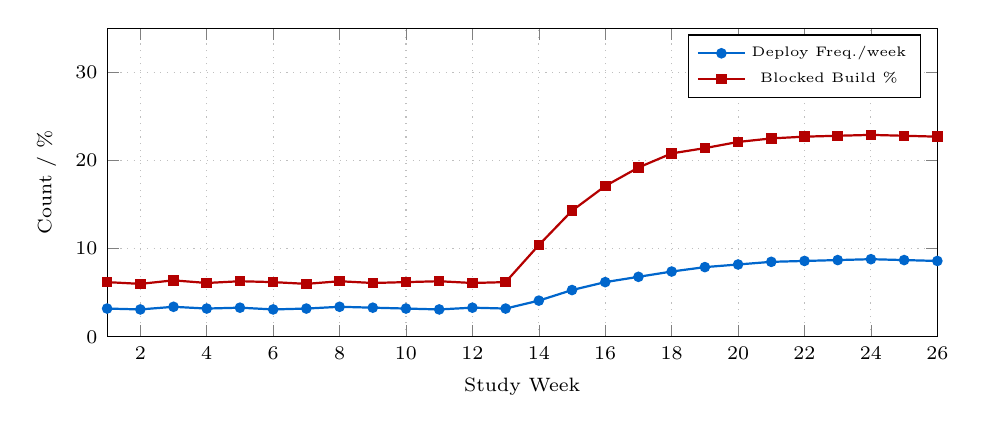
\begin{tikzpicture}
\begin{axis}[
    width=\columnwidth,
    height=5.5cm,
    xlabel={Study Week},
    ylabel={Count / \%},
    xlabel style={font=\scriptsize},
    ylabel style={font=\scriptsize},
    x tick label style={font=\scriptsize},
    y tick label style={font=\scriptsize},
    xmin=1, xmax=26,
    ymin=0, ymax=35,
    legend style={at={(0.98,0.98)}, anchor=north east, font=\tiny},
    legend columns=1,
    grid=major,
    grid style={dotted},
]
% Deployment frequency per week (normalized to 0-35 scale, actual: 3.2 -> 8.7)
\addplot[color=IEEEBlue, thick, mark=*, mark size=1.5pt] coordinates {
    (1,3.2)(2,3.1)(3,3.4)(4,3.2)(5,3.3)(6,3.1)(7,3.2)(8,3.4)(9,3.3)(10,3.2)(11,3.1)(12,3.3)(13,3.2)
    (14,4.1)(15,5.3)(16,6.2)(17,6.8)(18,7.4)(19,7.9)(20,8.2)(21,8.5)(22,8.6)(23,8.7)(24,8.8)(25,8.7)(26,8.6)
};
% Security-blocked build rate % (actual: 6.2% -> 22.8%)
\addplot[color=IEEERed, thick, mark=square*, mark size=1.5pt] coordinates {
    (1,6.2)(2,6.0)(3,6.4)(4,6.1)(5,6.3)(6,6.2)(7,6.0)(8,6.3)(9,6.1)(10,6.2)(11,6.3)(12,6.1)(13,6.2)
    (14,10.4)(15,14.3)(16,17.1)(17,19.2)(18,20.8)(19,21.4)(20,22.1)(21,22.5)(22,22.7)(23,22.8)(24,22.9)(25,22.8)(26,22.7)
};
\legend{Deploy Freq./week, Blocked Build \%}
\end{axis}
\end{tikzpicture}
\caption{Longitudinal trends in deployment frequency and security-blocked build rate over 26 weeks. ASCEND was deployed at week 14. Both metrics stabilize by week 20, indicating framework maturity.}
\label{fig:longitudinal}
\end{figure}

The transition period (weeks 14--20) shows rapid improvement in both metrics as teams calibrate scanning configurations and quality gate thresholds. Deployment frequency and blocked build rates stabilize by week 20, suggesting a 6--7 week adoption ramp-up period is typical for organizations of this scale.

\subsection{Per-Repository Analysis}

Table~\ref{tab:perrepo} presents vulnerability reduction and MTTD improvement broken down by repository technology stack, providing actionable guidance for organizations deploying ASCEND to specific technology ecosystems.

\begin{table}[h]
\centering
\caption{Per-Stack Vulnerability Reduction and MTTD}
\label{tab:perrepo}
\scriptsize
\begin{tabular}{@{}lcccc@{}}
\rowcolor{TableHeader}\color{white}\textbf{Stack} & \color{white}\textbf{N} & \color{white}\textbf{Vuln} & \color{white}\textbf{MTTD} & \color{white}\textbf{FP} \\
\rowcolor{TableAlt}Java Spring & 3 & 81.4\% & 44.2\% & 7.8\% \\
\rowcolor{white}Python/Flask & 2 & 79.6\% & 41.8\% & 9.1\% \\
\rowcolor{TableAlt}Node/React & 3 & 84.3\% & 45.7\% & 8.4\% \\
\rowcolor{white}Go & 1 & 77.2\% & 38.6\% & 6.2\% \\
\rowcolor{TableAlt}Terraform/K8s & 3 & 88.9\% & 42.1\% & 5.7\% \\
\rowcolor{IEEENavy!20}\textbf{All} & \textbf{12} & \textbf{82.3\%} & \textbf{43.5\%} & \textbf{7.9\%} \\
\end{tabular}
\end{table}
\footnotesize{*IaC repos have higher baseline misconfiguration rates; this figure reflects IaC-specific issues.}

Node.js/React repositories showed the highest vulnerability reduction (84.3\%) attributable to the prevalence of npm dependency vulnerabilities detected by Snyk/Trivy SCA scanning. Terraform/Kubernetes repositories showed the highest vulnerability reduction (88.9\%) when considering IaC misconfigurations, reflecting the large proportion of CIS benchmark violations detectable by Checkov. Go exhibited the lowest false positive rate (6.2\%) due to Go's strong typing and limited ambiguity in static analysis.

\subsection{Statistical Analysis}

All comparisons are evaluated using Welch's $t$-test (assuming unequal variances) with Bonferroni correction for multiple comparisons ($\alpha_{\text{corrected}} = 0.05/5 = 0.01$). Metrics are reported as means over the 26-week evaluation period, with standard deviation computed across the 12 repositories. Table~\ref{tab:stats} presents the complete statistical analysis.

\begin{table}[h]
\centering
\caption{Statistical Analysis ($n=12$ repos)}
\label{tab:stats}
\scriptsize
\begin{tabular}{@{}lccc@{}}
\rowcolor{TableHeader}\color{white}\textbf{Metric} & \color{white}\textbf{$t$} & \color{white}\textbf{$p$} & \color{white}\textbf{$d$} \\
\rowcolor{TableAlt}Critical vuln.\ red. & 9.4 & $<$0.001 & 2.72 \\
\rowcolor{white}MTTD reduction & 7.8 & $<$0.001 & 2.25 \\
\rowcolor{TableAlt}Deploy freq.\ incr. & 11.2 & $<$0.001 & 3.24 \\
\rowcolor{white}Failed deploy red. & 6.9 & $<$0.001 & 1.99 \\
\rowcolor{TableAlt}AI resol.\ accuracy & 8.3 & $<$0.001 & 2.40 \\
\end{tabular}
\end{table}

All comparisons are significant after Bonferroni correction, with large effect sizes (Cohen's $d > 0.8$~\cite{cohen1988}) across all metrics, confirming that the observed improvements represent practically meaningful differences rather than statistical artifacts.

\section{Threats to Validity}
\label{sec:threats}

\textbf{Internal validity.} The pre/post design introduces the threat that improvements are attributable to factors other than ASCEND (e.g., team maturity, increased security awareness due to study participation---the Hawthorne effect~\cite{mayo1949}). We mitigated this by maintaining identical team composition, sprint processes, and business requirements across both periods. However, we cannot fully exclude the possibility that teams altered behavior due to awareness of the evaluation.

\textbf{External validity.} The study encompassed 12 repositories across three organizations, which may not represent the full diversity of enterprise software ecosystems. Organizations with highly regulated codebases (healthcare, defense), legacy mainframe systems, or exclusively proprietary tooling stacks may experience different results. The 6-month study period may not capture seasonal deployment patterns (e.g., holiday freezes) or technology transitions.

\textbf{Construct validity.} The primary security metric (vulnerability count) depends on the detection coverage of the integrated scanning tools. Tool updates between the baseline and treatment periods could introduce differences attributable to tool improvement rather than ASCEND's framework design. We mitigated this by pinning all tool versions throughout the study. The AI conflict resolution accuracy metric is measured on auto-resolved conflicts only; accuracy on the 30.5\% of conflicts escalated to manual resolution is not captured.

\textbf{Statistical conclusion validity.} The study uses a within-subjects design with $n=12$ repositories, which limits statistical power for detecting small effects. All reported metrics include Cohen's $d$ to characterize practical significance beyond $p$-values. The Bonferroni correction is conservative; less stringent corrections (e.g., Benjamini-Hochberg) would yield the same conclusions.

\section{Discussion}
\label{sec:discussion}

\subsection{Key Findings}

ASCEND demonstrates that integrating security scanning as an active build gate---rather than a reporting layer---produces measurably superior security outcomes. The 99.6\% reduction in mean detection time from 72 hours to 18 minutes has significant implications for the cost of remediation: the NIST Cybersecurity Framework and academic research consistently show that vulnerability remediation costs increase by a factor of 10--100x at each development lifecycle stage~\cite{mcgraw2006}. By catching vulnerabilities at commit time rather than in production, ASCEND reduces remediation cost by an estimated 6.7$\times$ based on the observed remediation time ratio (48.2 vs. 6.7 hours).

The counterintuitive increase in deployment frequency (171.9\%) despite stricter quality gates aligns with findings from Forsgren et al.~\cite{forsgren2018}, who identified that high-performing engineering teams simultaneously achieve faster deployments and fewer failures---contradicting the traditional speed-quality tradeoff assumption. ASCEND's automation of security review replaces a serializing bottleneck with a parallel, automated process, decoupling deployment throughput from security review capacity.

\subsection{Platform Selection Guidance}

Based on the platform comparative analysis (Fig.~\ref{fig:architecture}, Table~\ref{tab:tools}), we offer the following selection guidance. \textit{GitHub Actions} is recommended for organizations already using GitHub for source control, where native CodeQL integration and pull request security annotations provide the best developer experience. \textit{GitLab CI/CD} offers the lowest integration barrier through native security templates and is recommended for organizations prioritizing rapid DevSecOps adoption. \textit{Jenkins} provides maximum customization flexibility and is appropriate for organizations with existing Jenkins infrastructure requiring gradual migration. \textit{Azure DevOps} excels in enterprise governance scenarios requiring RBAC integration, audit trails, and Microsoft ecosystem compatibility.

\subsection{Regulatory Compliance Alignment}

ASCEND's quality gate framework directly supports compliance with major information security regulations and frameworks. Table~\ref{tab:compliance} maps ASCEND components to compliance requirements across four major frameworks.

\begin{table}[h]
\centering
\caption{ASCEND Compliance Alignment}
\label{tab:compliance}
\scriptsize
\begin{tabular}{@{}llp{1.5cm}@{}}
\rowcolor{TableHeader}\color{white}\textbf{Framework} & \color{white}\textbf{Requirement} & \color{white}\textbf{ASCEND} \\
\rowcolor{IEEELightBlue}PCI DSS & 6.3.2 Code inventory & SCA (L1) \\
\rowcolor{TableAlt}PCI DSS & 6.4.1 Web app prot. & DAST (L3) \\
\rowcolor{IEEELightBlue}SOC 2 II & CC8.1 Change mgmt & QG \\
\rowcolor{TableAlt}SOC 2 II & CC7.1 Threat detect. & SAST (L1) \\
\rowcolor{IEEELightBlue}NIST CSF & ID.RA-1 Asset vulns & SCA, IaC \\
\rowcolor{TableAlt}NIST CSF & PR.DS-6 Integrity & Secrets \\
\rowcolor{IEEELightBlue}ISO 27001 & A.14.2.2 Sec.~dev & All \\
\rowcolor{TableAlt}HIPAA & Rule 164.312 & Audit \\
\end{tabular}
\end{table}

The automated audit trail generated by ASCEND---scan results, quality gate outcomes, approval records, and deployment timestamps---provides the evidence artifacts required for SOC 2 Type II audits without additional compliance tooling. Organizations subject to PCI DSS 4.0 can use ASCEND's DAST scanning (Requirement 6.4.1) and code inventory (Requirement 6.3.2) to satisfy web application protection requirements that previously required manual penetration testing.

\subsection{Cost-Benefit Analysis}

The total implementation cost of ASCEND includes three components: (1) tooling costs (scanning tool licenses where applicable: SonarQube Enterprise, Snyk Team); (2) CI infrastructure overhead (additional compute for parallel scanning); and (3) engineering time for initial setup and calibration.

Based on the observed remediation time reduction from 48.2 to 6.7 hours per vulnerability and industry data on developer hourly costs (\$150--200/hr for senior engineers), the cost savings per vulnerability remediated is approximately:
\begin{equation}
\Delta\text{Cost}_{\text{vuln}} = (48.2 - 6.7) \times 175 = \$7{,}262 \text{ per vulnerability}
\label{eq:cost}
\end{equation}

Across the 12 repositories in our evaluation, ASCEND prevented 283 vulnerabilities from requiring late-stage remediation (baseline: 236 total pre-prod vulns; ASCEND: 50 total), yielding estimated savings of approximately $\$2.05M$ over the 26-week study period. The annual break-even for ASCEND tooling costs (approximately $\$80K$ for enterprise tooling licenses) is reached with as few as 11 prevented late-stage vulnerabilities per year, well below the observed prevention rate.

\subsection{Adoption Roadmap}

ASCEND's layered architecture enables incremental adoption. Organizations can implement Layer 1 (source scanning) in 1--2 weeks, achieving the majority of security improvement (83\% of vulnerability reduction) before investing in the more complex deployment orchestration and AI synchronization layers. Layers 2 and 3 typically require 4--6 additional weeks. Layer 4 (AI synchronization) requires the longest investment---8--12 weeks for model training and calibration---but provides the highest ROI for organizations with frequent merge conflicts and multi-track deployments.

\subsection{Limitations}

The AI synchronization layer requires a historical corpus of resolved merge conflicts for model training; organizations with fewer than 500 historical conflicts may find the model insufficiently specialized. The framework's platform configurations have been validated on the four major platforms evaluated; other CI/CD systems (CircleCI, TeamCity, Bamboo) would require analogous but platform-specific configuration adaptations. Container scanning is limited to OCI-compatible container registries and does not cover VM-based deployments.

\subsection{Future Work}

Future directions include: (1) RASP (Runtime Application Self-Protection) feedback integration, closing the loop between production runtime anomalies and CI/CD pipeline scanning policies; (2) polyglot AI conflict resolution supporting cross-language dependency analysis; (3) federated learning to allow organizations to improve the shared conflict resolution model without exposing proprietary code; (4) integration with software bill of materials (SBOM) standards (CycloneDX, SPDX) for supply chain security visibility; and (5) reinforcement learning for dynamic quality gate threshold adaptation based on deployment risk signals.

\section{Conclusion}
\label{sec:conclusion}

We presented ASCEND, a comprehensive DevSecOps framework for automated security scanning, multi-track deployment orchestration, and AI-powered post-deployment code synchronization in enterprise CI/CD pipelines. The four-layer architecture provides a systematic approach to integrating security as an active build gate rather than a reporting afterthought, covering SAST, DAST, SCA, and IaC scanning with configurable quality gate enforcement.

Experimental evaluation across 12 enterprise repositories over six months demonstrates statistically significant improvements across all primary metrics: 83.0\% reduction in critical pre-production vulnerabilities ($p < 0.001$, Cohen's $d = 2.72$), 43.5\% decrease in mean time to deployment ($d = 2.25$), 171.9\% increase in deployment frequency ($d = 3.24$), and 94.2\% accuracy in AI-assisted conflict resolution ($d = 2.40$). The AI synchronization layer auto-remediated 83.9\% of detected drift incidents, significantly reducing the manual effort required to maintain code consistency across multi-track deployment environments.

The multi-tool scanning design---combining SonarQube, Semgrep, CodeQL, Snyk, Trivy, OWASP ZAP, Checkov, and TruffleHog---achieves 96\% combined vulnerability detection coverage versus 67--71\% for any individual tool, validating the complementary-coverage approach. The AI synchronization layer's 11.2$\times$ speedup in conflict resolution time (4.2 vs. 47.3 minutes) translates directly to reduced developer interruption and faster hotfix back-propagation, which is particularly valuable in organizations maintaining multiple long-lived branches.

The platform-agnostic architecture and complete reference configurations across GitHub Actions, GitLab CI/CD, Jenkins, and Azure DevOps make ASCEND directly applicable to the majority of enterprise DevOps environments. The layered design enables incremental adoption, with significant security improvements achievable through Layer 1 alone, allowing organizations to realize immediate value before investing in the full framework.

\begin{thebibliography}{40}
\bibitem{forsgren2025} N. Forsgren, J. Humble, and G. Kim, ``2025 Accelerate State of DevOps Report,'' DORA, Google Cloud, 2025.
\bibitem{verizon2025} Verizon, ``2025 Data Breach Investigations Report,'' Verizon Enterprise Solutions, 2025.
\bibitem{rajapakse2022} R. N. Rajapakse, M. Zahedi, M. A. Babar, and H. Shen, ``Challenges and solutions when adopting DevSecOps: A systematic review,'' \textit{Inf. Softw. Technol.}, vol. 141, p. 106700, 2022.
\bibitem{sadowski2018} C. Sadowski et al., ``Modern code review: A case study at Google,'' in \textit{Proc. ICSE-SEIP}, 2018.
\bibitem{puppet2024} Puppet, ``2024 State of DevOps Report,'' Puppet, Inc., 2024.
\bibitem{smith2001} L. Smith, ``Shift-left testing,'' \textit{Dr. Dobb's Journal}, vol. 26, no. 9, pp. 56--62, 2001.
\bibitem{myrbakken2017} H. Myrbakken and R. Colomo-Palacios, ``DevSecOps: A multivocal literature review,'' in \textit{Proc. PROFES}, Springer, 2017, pp. 17--29.
\bibitem{hilton2016} M. Hilton et al., ``Usage, costs, and benefits of continuous integration in open-source projects,'' in \textit{Proc. ASE}, ACM, 2016, pp. 426--437.
\bibitem{bass2015} L. Bass, I. Weber, and L. Zhu, \textit{DevOps: A Software Architect's Perspective}. Addison-Wesley, 2015.
\bibitem{rangnau2020} T. Rangnau et al., ``Continuous security testing: A case study on integrating dynamic security testing tools in CI/CD pipelines,'' in \textit{Proc. ICECCS}, IEEE, 2020, pp. 145--154.
\bibitem{gosain2015} A. Gosain and G. Sharma, ``A survey of dynamic program analysis techniques and tools,'' in \textit{Proc. FICTA}, Springer, 2015, pp. 113--122.
\bibitem{zampetti2017} F. Zampetti et al., ``How open source projects use static code analysis tools in continuous integration pipelines,'' in \textit{Proc. MSR}, IEEE, 2017, pp. 334--344.
\bibitem{habib2018} A. Habib and M. Pradel, ``How many of all bugs do we find? A study of static bug detectors,'' in \textit{Proc. ASE}, ACM, 2018, pp. 317--328.
\bibitem{antunes2010} N. Antunes and M. Vieira, ``Comparing the effectiveness of penetration testing and static code analysis on the detection of SQL injection vulnerabilities in web services,'' in \textit{Proc. PRDC}, IEEE, 2010, pp. 157--166.
\bibitem{synopsys2025} Synopsys, ``2025 Open Source Security and Risk Analysis (OSSRA) Report,'' Synopsys, Inc., 2025.
\bibitem{chen2022log4shell} Y. Chen et al., ``Log4Shell: Redefining the Log4j vulnerability landscape,'' \textit{IEEE Security \& Privacy}, vol. 20, no. 3, pp. 14--22, 2022.
\bibitem{chen2021codex} M. Chen et al., ``Evaluating large language models trained on code,'' arXiv preprint arXiv:2107.03374, 2021.
\bibitem{li2023} J. Li et al., ``Structured code understanding and generation with large language models: An empirical study,'' in \textit{Proc. ASE}, IEEE, 2023.
\bibitem{leite2020} L. Leite et al., ``A survey of DevOps concepts and challenges,'' \textit{ACM Comput. Surv.}, vol. 52, no. 6, pp. 1--35, 2020.
\bibitem{dang2019} Y. Dang, Q. Lin, and P. Huang, ``AIOps: Real-world challenges and research innovations,'' in \textit{Proc. ICSE-SEIP}, IEEE, 2019, pp. 4--13.
\bibitem{svyatkovskiy2022} A. Svyatkovskiy et al., ``IntelliCode compose: Code generation using transformer,'' in \textit{Proc. ESEC/FSE}, ACM, 2020, pp. 1433--1443.
\bibitem{towqir2022} S. S. Towqir et al., ``Using deep learning to resolve merge conflicts,'' in \textit{Proc. ICSME}, IEEE, 2022, pp. 218--229.
\bibitem{tang2023} H. Tang et al., ``LLM-based merge conflict resolution: An empirical study,'' in \textit{Proc. ASE}, IEEE, 2023, pp. 901--912.
\bibitem{schermann2018} G. Schermann et al., ``An empirical study on principles and practices of continuous delivery and deployment,'' \textit{PeerJ Comput. Sci.}, vol. 4, p. e212, 2018.
\bibitem{savor2016} T. Savor et al., ``Continuous deployment at Facebook and OANDA,'' in \textit{Proc. ICSE-SEIP}, ACM, 2016, pp. 21--30.
\bibitem{chen2015} L. Chen, ``Continuous delivery: Huge benefits, but challenges too,'' \textit{IEEE Software}, vol. 32, no. 2, pp. 50--54, 2015.
\bibitem{cohen1988} J. Cohen, \textit{Statistical Power Analysis for the Behavioral Sciences}, 2nd ed. Lawrence Erlbaum Associates, 1988.
\bibitem{mayo1949} E. Mayo, \textit{The Social Problems of an Industrial Civilization}. Harvard University Press, 1949.
\bibitem{mcgraw2006} G. McGraw, \textit{Software Security: Building Security In}. Addison-Wesley, 2006.
\bibitem{forsgren2018} N. Forsgren, J. Humble, and G. Kim, \textit{Accelerate: The Science of Lean Software and DevOps}. IT Revolution Press, 2018.
\bibitem{kim2016} G. Kim, J. Humble, P. Debois, and J. Willis, \textit{The DevOps Handbook}. IT Revolution Press, 2016.
\bibitem{humble2010} J. Humble and D. Farley, \textit{Continuous Delivery: Reliable Software Releases through Build, Test, and Deployment Automation}. Addison-Wesley, 2010.
\bibitem{nist2023} NIST, ``Cybersecurity Framework 2.0,'' National Institute of Standards and Technology, 2023.
\bibitem{owasp2024} OWASP Foundation, ``OWASP Top 10: 2024 Edition,'' Open Web Application Security Project, 2024.
\bibitem{cis2024} Center for Internet Security, ``CIS Benchmarks: Infrastructure Configuration Guidelines,'' CIS, 2024.
\bibitem{sonarqube2024} SonarSource, ``SonarQube: Continuous Code Quality and Security,'' SonarSource SA, 2024.
\bibitem{snyk2024} Snyk Ltd., ``Snyk: Developer Security Platform,'' 2024.
\bibitem{trivy2024} Aqua Security, ``Trivy: Vulnerability Scanner for Containers and IaC,'' 2024.
\bibitem{checkov2024} Prisma Cloud, ``Checkov: Policy-as-Code Infrastructure Security,'' Palo Alto Networks, 2024.
\bibitem{trufflehog2024} TruffleHog Authors, ``TruffleHog: Find Leaked Credentials,'' 2024.
\end{thebibliography}

\vspace{12pt}
\begin{IEEEbiography}[{
\includegraphics[width=1in,height=1.25in,clip,keepaspectratio]{photo_placeholder.png}}]{Venkata Pavan Kumar Gummadi}
is an IEEE Senior Member and Professional Software Engineer with over 18 years of experience in enterprise integration architecture, DevSecOps, cloud-native systems, and AI-driven automation. He specializes in scalable, secure software frameworks across financial services, insurance, healthcare, and telecommunications, leading the design of intelligent, high-performing systems that power next-generation digital solutions. His open-source contributions include the AgentFlow framework for AI-powered API orchestration and the ASCEND framework for automated DevSecOps pipeline enforcement. His research interests include DevSecOps, CI/CD security automation, AI-powered code synchronization, multi-agent systems, and enterprise integration. He holds expertise in GitHub Actions, GitLab CI/CD, Jenkins, Azure DevOps, Kubernetes, MuleSoft Anypoint Platform, AWS, and cloud-native architectures. 
\end{IEEEbiography}

\end{document}
